\documentclass[12pt, oneside]{article}
\usepackage[letterpaper, margin=1in, headsep=0.5in]{geometry}
\usepackage[english]{babel}
\usepackage[utf8]{inputenc}
\usepackage{amsmath}
\usepackage{amsfonts}
\usepackage{amssymb}
\usepackage{tikz}
\usetikzlibrary{quotes, angles}
\usepackage{graphicx}
\usepackage{yhmath}
\usepackage{multicol}
%\usepackage{pgfplots}
%\pgfplotsset{width=10cm,compat=1.9}
%\usepgfplotslibrary{statistics}
%\usepackage{pgfplotstable}
%\usepackage{tkz-fct}
%\usepackage{venndiagram}

\usepackage{fancyhdr}
\pagestyle{fancy}
\fancyhf{}
\rhead{\thepage \\Name: \hspace{1.5in}.\\}
\lhead{BECA / Dr. Huson / 10th Grade Geometry\\* 31 May 2019}

\renewcommand{\headrulewidth}{0pt}

\begin{document}
\subsubsection*{Do Now: Construction \& similarity pre-quiz}
Use only a compass and straightedge for these classical constructions, showing all construction marks.
  \begin{enumerate}

  \item Bisect the given angle. \vspace{2cm}
    \begin{center}
    \begin{tikzpicture}
      \draw [<->, thick] (80:6)--(0,0)--(20:6);
      \draw [fill] (0,0) circle [radius=0.05] node[below]{$A$};
    \end{tikzpicture}
  \end{center} \vspace{0.5cm}

  \item Construct the perpendicular bisector to $\overline{AB}$.
    \vspace{3.5cm}
    \begin{center}
    \begin{tikzpicture}
      \draw [-, thick] (0,2)--(5,0);
      \draw [fill] (0,2) circle [radius=0.05] node[above left]{$A$};
      \draw [fill] (5,0) circle [radius=0.05] node[below right]{$B$};
    \end{tikzpicture}
  \end{center} \vspace{2cm}

\newpage

  \item Given the line $l$ and point $P$, construct the perpendicular to $l$ through $P$.\\
    \vspace{2cm}
    \begin{center}
    \begin{tikzpicture}
      \draw [<->, thick] (0,0)--(12,0)node[below]{$l$};
      \draw [fill] (5,2) circle [radius=0.05] node[above left]{$P$};
    \end{tikzpicture}
  \end{center} \vspace{3cm}

  \item Construct a perpendicular to $\overline{AB}$ though $C$.\\
    %\hspace{1cm} Given the line  $l$ and point $P$.
    \vspace{2cm}
    \begin{center}
    \begin{tikzpicture}
      \draw [<->, thick] (0,0)--(11,0)--(6,3)--cycle;
      \draw [fill] (0,0) circle [radius=0.05] node[left]{$A$};
      \draw [fill] (11,0) circle [radius=0.05] node[right]{$B$};
      \draw [fill] (6,3) circle [radius=0.05] node[above right]{$C$};
    \end{tikzpicture}
  \end{center} \vspace{5cm}

\newpage

  \begin{multicols}{2}[\item Given $\overline{APJ}$ and $\overline{KPB}$ as shown below. $\overline{AB} \parallel \overline{JK}$. $AP=4.8$, $JP=12$, and $BP=2.2$. \vspace{0.5cm} ]
    \begin{enumerate}
      \item $\triangle ABP \sim$ \rule{2cm}{0.15mm} \vspace{0.7cm}
      \item $\overline{AP} \rightarrow$ \rule{2cm}{0.15mm} \vspace{0.7cm}
      \item $\overline{BP} \rightarrow$ \rule{2cm}{0.15mm}
      \item What is the scale factor?\\[0.7cm] $k=$  \rule{1.2cm}{0.15mm} $=$ \vspace{0.7cm}
      \item Find $KP$. \vspace{1cm}
    \end{enumerate}
    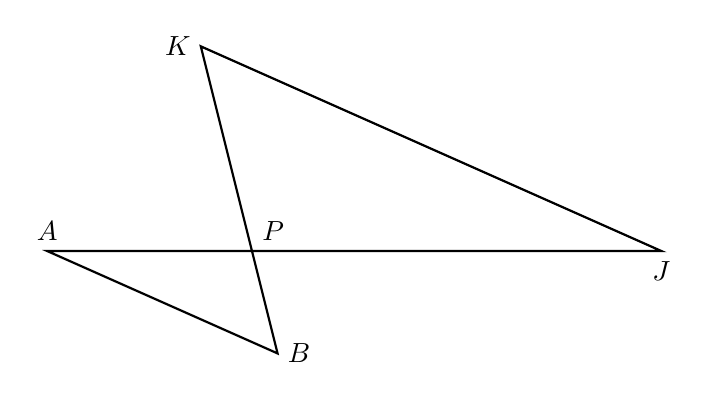
\begin{tikzpicture}[scale=1.3]
        \draw [thick]
          (0.25,-1)node[right]{$B$}--
          (-0.5,2)node[left]{$K$}--
          (4,0)node[below]{$J$}--
          (0,0)node[above right]{$P$}--
          (-2,0)node[above]{$A$}--cycle;
      \end{tikzpicture}
   \end{multicols} \vspace{1.5cm}

 \begin{multicols}{2}[\item Given, the diagram below, with $\overline{ABD}$, $\overline{ACE}$, and $\angle ABC \cong \angle AED$. $AB=10$, $AC=8$, and $AD=14$. \vspace{0.5cm} ]
     \begin{enumerate}
       \item $\triangle ABC \sim$ \rule{2cm}{0.15mm} \vspace{1cm}
       \item $\overline{AB} \rightarrow$ \rule{2cm}{0.15mm} \vspace{1cm}
       \item $\overline{AC} \rightarrow$ \rule{2cm}{0.15mm}
       \item What is the scale factor?\\[1cm] $k=$  \rule{1.2cm}{0.15mm} $=$ \vspace{1cm}
       \item Find $AE$.\vspace{1cm}
     \end{enumerate}
      \begin{tikzpicture}[scale=.5]
        \draw [thick]
        (0,0) node[above right] {$A$}--
        (230:17.5) node[below left] {$E$}--
        (260:14) node[below right] {$D$}--cycle;
        \draw [thick]
        (230:8) node[above left] {$C$}--
        (260:10) node[right] {$B$}--cycle;
      \end{tikzpicture}
    \end{multicols} \vspace{2cm}

\newpage

  \begin{multicols}{2}[
    \item In the diagram below, the chords $\overline{AE}$ and $\overline{BD}$ intersect at $C$. Given that $AC=5$, $BC=4$, and $CE=10$. The arc measure of $m \wideparen{AD}=170^\circ$. %uses yhmath
    \vspace{0.5cm}
      ]
    \begin{enumerate}
      \item $\triangle ABC \sim$ \rule{2cm}{0.15mm} \vspace{0.7cm}
      \item $\overline{AC} \rightarrow$ \rule{2cm}{0.15mm} \vspace{0.7cm}
      \item $\overline{BC} \rightarrow$ \rule{2cm}{0.15mm}
      \item What is the scale factor?\\[1cm] $k=$  \rule{1.2cm}{0.15mm} $=$ \vspace{0.7cm}
      \item Find $CD$. \vspace{1cm}
    \end{enumerate}
      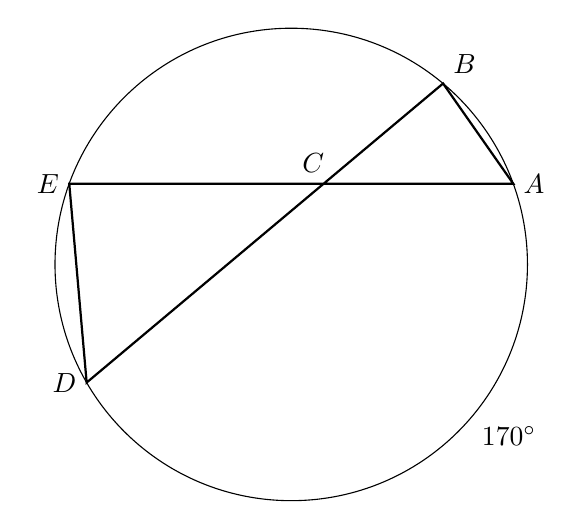
\begin{tikzpicture}[scale=.6]
        \draw (0,0) circle[radius=5];
        \draw [thick]
        (20:5) node[right] {$A$}--
        (160:5) node[left] {$E$}--
        (210:5) node[left] {$D$}--
        (50:5) node[above right] {$B$}--cycle;
        \draw (75:1.8) node[above] {$C$};
        \node at (320:5)[below right]{$170^\circ$};
      \end{tikzpicture}
   \end{multicols} \vspace{1.5cm}

   \begin{multicols}{2}[
     \item In the diagram below, the chords $\overline{AE}$ and $\overline{BD}$ intersect at $C$. Given that $AC=6$, $BC=9$, and $CE=12$.
     \vspace{0.5cm}
       ]
     \begin{enumerate}
       \item $\triangle ABC \sim$ \rule{2cm}{0.15mm} \vspace{0.7cm}
       \item $\overline{AC} \rightarrow$ \rule{2cm}{0.15mm} \vspace{0.7cm}
       \item $\overline{BC} \rightarrow$ \rule{2cm}{0.15mm}
       \item What is the scale factor?\\[1cm] $k=$  \rule{1.2cm}{0.15mm} $=$ \vspace{0.7cm}
       \item Find $CD$. \vspace{1cm}
     \end{enumerate}
       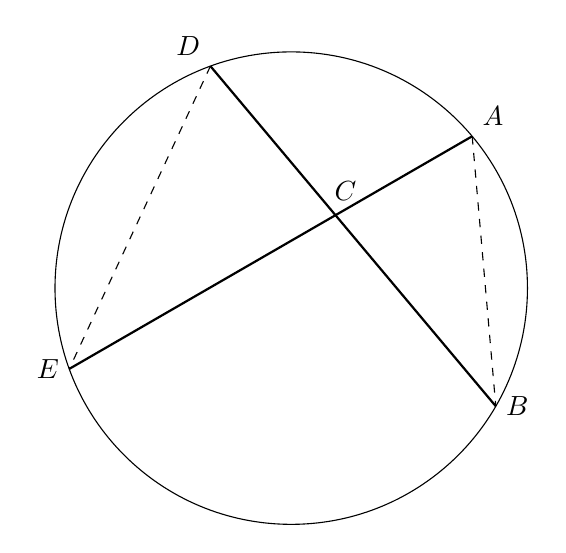
\begin{tikzpicture}[scale=.6]
        \draw (0,0) circle[radius=5];
        \draw [thick]
          (40:5) node[above right] {$A$}--
          (200:5) node[left] {$E$};
        \draw [dashed] (40:5) -- (-30:5);
        \draw [thick]
          (-30:5) node[right] {$B$}--
          (110:5) node[above left] {$D$};
        \draw [dashed] (110:5) -- (200:5);
        \draw (55:2) node[above] {$C$};
       \end{tikzpicture}
    \end{multicols}

\end{enumerate}
\newpage
\setcounter{page}{1}
\subsubsection*{Exit Note: Construction \& similarity quiz}
Use only a compass and straightedge for these classical constructions, showing all construction marks.
  \begin{enumerate}

  \item Bisect the given angle. \vspace{2cm}
    \begin{center}
    \begin{tikzpicture}
      \draw [<->, thick] (80:6)--(0,0)--(20:6);
      \draw [fill] (0,0) circle [radius=0.05] node[below]{$A$};
    \end{tikzpicture}
  \end{center} \vspace{0.5cm}

  \item Construct the perpendicular bisector to $\overline{AB}$.
    \vspace{3.5cm}
    \begin{center}
    \begin{tikzpicture}
      \draw [-, thick] (0,2)--(5,0);
      \draw [fill] (0,2) circle [radius=0.05] node[above left]{$A$};
      \draw [fill] (5,0) circle [radius=0.05] node[below right]{$B$};
    \end{tikzpicture}
  \end{center} \vspace{2cm}

\newpage

  \item Given the line $l$ and point $P$, construct the perpendicular to $l$ through $P$.\\
    \vspace{2cm}
    \begin{center}
    \begin{tikzpicture}
      \draw [<->, thick] (0,0)--(12,0)node[below]{$l$};
      \draw [fill] (5,2) circle [radius=0.05] node[above left]{$P$};
    \end{tikzpicture}
  \end{center} \vspace{3cm}

  \item Construct a perpendicular to $\overline{AB}$ though $C$.\\
    %\hspace{1cm} Given the line  $l$ and point $P$.
    \vspace{2cm}
    \begin{center}
    \begin{tikzpicture}
      \draw [<->, thick] (0,0)--(11,0)--(6,3)--cycle;
      \draw [fill] (0,0) circle [radius=0.05] node[left]{$A$};
      \draw [fill] (11,0) circle [radius=0.05] node[right]{$B$};
      \draw [fill] (6,3) circle [radius=0.05] node[above right]{$C$};
    \end{tikzpicture}
  \end{center} \vspace{5cm}

\newpage

  \begin{multicols}{2}[\item Given $\overline{APJ}$ and $\overline{KPB}$ as shown below. $\overline{AB} \parallel \overline{JK}$. $AP=4.8$, $JP=12$, and $BP=2.2$. \vspace{0.5cm} ]
    \begin{enumerate}
      \item $\triangle ABP \sim$ \rule{2cm}{0.15mm} \vspace{0.7cm}
      \item $\overline{AP} \rightarrow$ \rule{2cm}{0.15mm} \vspace{0.7cm}
      \item $\overline{BP} \rightarrow$ \rule{2cm}{0.15mm}
      \item What is the scale factor?\\[1cm] $k=$  \rule{1.2cm}{0.15mm} $=$ \vspace{0.7cm}
      \item Find $KP$. \vspace{1cm}
    \end{enumerate}
    \begin{tikzpicture}[scale=1.4]
        \draw [thick]
          (0.25,-1)node[right]{$B$}--
          (-0.5,2)node[left]{$K$}--
          (4,0)node[right]{$J$}--
          (0,0)node[above right]{$P$}--
          (-2,0)node[left]{$A$}--cycle;
      \end{tikzpicture}
   \end{multicols} \vspace{1.5cm}

 \begin{multicols}{2}[\item Given, the diagram below, with $\overline{ABD}$, $\overline{ACE}$, and $\angle ABC \cong \angle AED$. $AB=10$, $AC=8$, and $AD=14$. \vspace{0.5cm} ]
     \begin{enumerate}
       \item $\triangle ABC \sim$ \rule{2cm}{0.15mm} \vspace{1cm}
       \item $\overline{AB} \rightarrow$ \rule{2cm}{0.15mm} \vspace{1cm}
       \item $\overline{AC} \rightarrow$ \rule{2cm}{0.15mm} \vspace{1cm}
       \item What is the scale factor?\\[1cm] $k=$  \rule{1.2cm}{0.15mm} $=$ \vspace{1cm}
       \item Find $AE$.\vspace{1cm}
     \end{enumerate}
      \begin{tikzpicture}[scale=.5]
        \draw [thick]
        (0,0) node[above right] {$A$}--
        (230:17.5) node[below left] {$E$}--
        (260:14) node[below right] {$D$}--cycle;
        \draw [thick]
        (230:8) node[above left] {$C$}--
        (260:10) node[right] {$B$}--cycle;
      \end{tikzpicture}
    \end{multicols} \vspace{2cm}

\newpage

  \begin{multicols}{2}[
    \item In the diagram below, the chords $\overline{AE}$ and $\overline{BD}$ intersect at $C$. Given that $AC=5$, $BC=4$, and $CE=10$. The arc measure of $m \wideparen{AD}=170^\circ$. %uses yhmath
    \vspace{0.5cm}
      ]
    \begin{enumerate}
      \item $\triangle ABC \sim$ \rule{2cm}{0.15mm} \vspace{0.7cm}
      \item $\overline{AC} \rightarrow$ \rule{2cm}{0.15mm} \vspace{0.7cm}
      \item $\overline{BC} \rightarrow$ \rule{2cm}{0.15mm}
      \item What is the scale factor?\\[1cm] $k=$  \rule{1.2cm}{0.15mm} $=$ \vspace{0.7cm}
      \item Find $CD$. \vspace{1cm}
    \end{enumerate}
      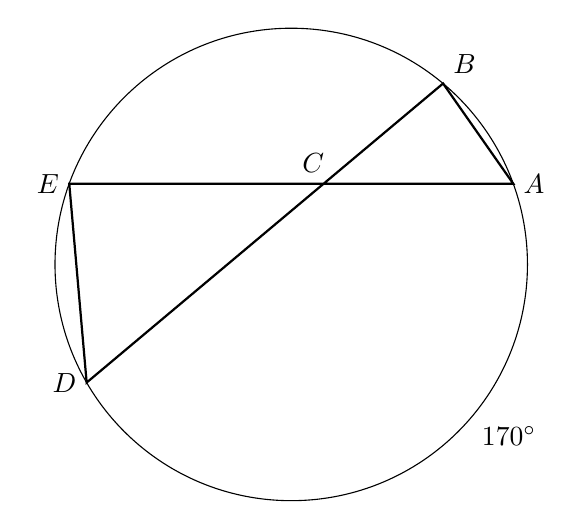
\begin{tikzpicture}[scale=.6]
        \draw (0,0) circle[radius=5];
        \draw [thick]
        (20:5) node[right] {$A$}--
        (160:5) node[left] {$E$}--
        (210:5) node[left] {$D$}--
        (50:5) node[above right] {$B$}--cycle;
        \draw (75:1.8) node[above] {$C$};
        \node at (320:5)[below right]{$170^\circ$};
      \end{tikzpicture}
   \end{multicols} \vspace{1.5cm}

   \begin{multicols}{2}[
     \item In the diagram below, the chords $\overline{AE}$ and $\overline{BD}$ intersect at $C$. Given that $AC=6$, $BC=9$, and $CE=12$.
     \vspace{0.5cm}
       ]
     \begin{enumerate}
       \item $\triangle ABC \sim$ \rule{2cm}{0.15mm} \vspace{0.7cm}
       \item $\overline{AC} \rightarrow$ \rule{2cm}{0.15mm} \vspace{0.7cm}
       \item $\overline{BC} \rightarrow$ \rule{2cm}{0.15mm}
       \item What is the scale factor?\\[1cm] $k=$  \rule{1.2cm}{0.15mm} $=$ \vspace{0.7cm}
       \item Find $CD$. \vspace{1cm}
     \end{enumerate}
       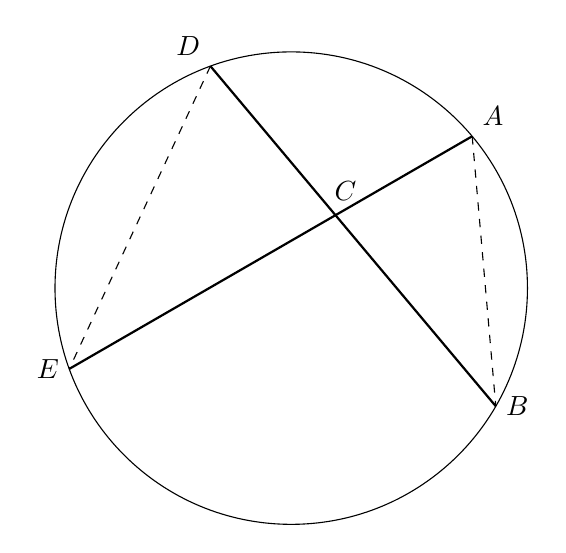
\begin{tikzpicture}[scale=.6]
        \draw (0,0) circle[radius=5];
        \draw [thick]
          (40:5) node[above right] {$A$}--
          (200:5) node[left] {$E$};
        \draw [dashed] (40:5) -- (-30:5);
        \draw [thick]
          (-30:5) node[right] {$B$}--
          (110:5) node[above left] {$D$};
        \draw [dashed] (110:5) -- (200:5);
        \draw (55:2) node[above] {$C$};
       \end{tikzpicture}
    \end{multicols}

\end{enumerate}
\end{document}
